%%%%%%%%%%%%%%%%%%%%%%%%%%%%%%%%%%%%%%%%%%%%%%%%%%%%%%%%%%%%%%%%%%%%%%%%%%%%%%%%%%%%%%%%%%%%%%%%%%%%%%%%%%%%%%%%%%%%%%%%%%%%%%%%%%%%%%%%%%%%%%%%%%%%%%%%%%%%%%%%%%%%%%%%%%%%%%%%%%%%%%%%%%%%%%%%%%%%%%%%%%%%%%%%%%%%%%%%%%%%%%%%%%%%%%%%%%%%%%%%%%%%%%%%%%%%%%%%%%%%%%%%%%%%%%%%%%%%%%%%%%%%%%%%%%%%%%%%%%%%%%%%%%%%%%%%%%%%%%%%%%%%%%%%%%%%%%

\begin{frame}{}
    \begin{center}
        \Huge  Algunos resultados sobre la ``Descomposición de Jordan"  
    \end{center}
\end{frame}


%%%%%%%%%%%%%%%%%%%%%%%%%%%%%%%%%%%%%%%%%%%%%%%%%%%%%%%%%%%%%%%%%%%%%%%%%%%%%%%%%%%%%%%%%%%%%%%%%%%%%%%%%%%%%%%%%%%%%%%%%%%%%%%%%%%%%%%%%%%%%%%%%%%%%%%%%%%%%%%%%%%%%%%%%%%%%%%%%%%%%%%%%%%%%%%%%%%%%%%%%%%%%%%%%%%%%%%%%%%%%%%%%%%%%%%%%%%%%%%%%%%%%%%%%%%%%%%%%%%%%%%%%%%%%%%%%%%%%%%%%%%%%%%%%%%%%%%%%%%%

\begin{frame}{Condiciones necesarias para  la descomposición de Jordan}
\begin{itemize}
    \item \textbf{Definición:}
      \begin{block}{}
          Se dice que un espacio normado ordenado $X$ satisface la descomposición de Jordan si toda función de variación acotada $ g,h:[a,b]\to X$, existen $f:[a,b]\to X$ crecientes tales que $ f=g-h $.
      \end{block}
    \item \textbf{Lema}
\end{itemize}
    \begin{block}{}
        Si $f:[a,b]\to X$ cumple la descomposición de Jordan, entonces $f$ es orden acotado. 
    \end{block}
\end{frame}


%%%%%%%%%%%%%%%%%%%%%%%%%%%%%%%%%%%%%%%%%%%%%%%%%%%%%%%%%%%%%%%%%%%%%%%%%%%%%%%%%%%%%%%%%%%%%%%%%%%%%%%%%%%%%%%%%%%%%%%%%%%%%%%%%%%%%%%%%%%%%%%%%%%%%%%%%%%%%%%%%%%%%%%%%%%%%%%%%%%%%%%%%%%%%%%%%%%%%%%%%%%%%%%%%%%%%%%%%%%%%%%%%%%%%%%%%%%%%%%%%%%%%%%%%%%%%%%%%%%%%%%%%%%%%%%%%%%%%%%%%%%%%%%%%%%%%%%%%%%%

    \begin{frame}{}
        \begin{block}{Teorema}
            Sea $X$ un ENO. Si $P$ no es generador, entonces existe  $f : [a,b] \longrightarrow X $  de variación acotada y que no cumple la descomposición de Jordan.
        \end{block}
        Demostración: Sea $ x_{0} \in X  $ tal que $ x_{0} \notin P - P $. Se define $ f: [a,b] \longrightarrow X $ 
        
        \[ f(t) = \left\{ \begin{array}{lcc}
             2 x_{0} , &   si  &  t=b , \\
             \\  x_{0} , &  si & t=a , \\
             \\ 0 ,  &  si  & t \in (a,b) . 
             \end{array}
   \right. \]
        Si existieran $g,h: [a,b] \longrightarrow X$ crecientes tal que $ f = g - h $ entonces 
        $ x_{0} = f(b) - f(a) = (g(b) - g(a) ) - ( h(b) - h(a)) . $
    \end{frame}

%%%%%%%%%%%%%%%%%%%%%%%%%%%%%%%%%%%%%%%%%%%%%%%%%%%%%%%%%%%%%%%%%%%%%%%%%%%%%%%%%%%%%%%%%%%%%%%%%%%%%%%%%%%%%%%%%%%%%%%%%%%%%%%%%%%%%%%%%%%%%%%%%%%%%%%%%%%%%%%%%%%%%%%%%%%%%%%%%%%%%%%%%%%%%%%%%%%%%%%%%%%%%%%%%%%%%%%%%%%%%%%%%%%%%%%%%%%%%%%%%%%%%%%%%%%%%%%%%%%%%%%%%%%%%%%%%%%%%%%%%%%%%%%%%%%%%%%%%%%%%%%%%%%%%

\begin{frame}{}
    \begin{itemize}
        \item \textbf{Ejemplo}
        \begin{block}{}
            	El espacio $(L_1[0,1], \|\cdot\|_1)$ con el orden usual de funciones. El cono $L_1[0,1]_+$ es generador ya que toda función en $L_1[0,1]$ es la diferencia de su parte positiva  parte negativa. Ver el ejemplo 2.5.1 en \cite{Gou2004}. %  shows $L_1[0,1]_+$ is an extensible cone.
        \end{block}
        \item \textbf{Función}
        \begin{block}{}
            Sea $f:[0,1] \longrightarrow L_1 [0,1]$  definida por  $f(0)=0$ (función nula) y para todo  $t \in (0,1]$, $f(t)=T_t$, donde $T_t:[0,1] \longrightarrow \mathbb{R}$ está dada por

	$$ T _t(s)=\left\{
	\begin{array}{ll}
		n_0 , & \hbox{$s\in[0,\frac{1}{(n_0 )^3}]$;} \\
		0, & \hbox{otherwise,}
	\end{array}
	\right.
	$$
donde $n_0 = [\frac{1}{t}]$.
        \end{block}
    \end{itemize}
\end{frame}


%%%%%%%%%%%%%%%%%%%%%%%%%%%%%%%%%%%%%%%%%%%%%%%%%%%%%%%%%%%%%%%%%%%%%%%%%%%%%%%%%%%%%%%%%%%%%%%%%%%%%%%%%%%%%%%%%%%%%%%%%%%%%%%%%%%%%%%%%%%%%%%%%%%%%%%%%%%%%%%%%%%%%%%%%%%%%%%%%%%%%%%%%%%%%%%%%%%%%%%%%%%%%%%%%%%%%%%%%%%%%%%%%%%%%%%%%%%%%%%%%%%%%%%%%%%%%%%%%%%%%%%%%%%%%%%%%%%%%%%%%%%%%%%%%%%%%%%%%%%%%%%%%%%%%

\begin{frame}{}
    	Let $P= \{t_0 =0, t_1, ... , t_{k}=1 \} \in \mathcal{P}[a,b] $ and $m_{i}= [\frac{1}{t_{i}}] \in \mathbb{N}  $ for all $i=1,...k.$ 
	Since $1= m_{n} \leq m_{n-1} \leq \cdots \leq m_{1}$, then 
	$ \frac{1}{(m_1)^3} \leq \frac{1}{(m_2)^3} \leq  \cdots \leq \frac{1}{(m_n)^3}=1  $.\\
	Define a set  $ \{ t'_{0}, t'_{1}, ... , t'_{n}  \}$ by $ t'_{0}=0, t'_{1}= t_{1} $ and $ t'_{j}= \min \{ t_{i} \in P- \{ 0 \}  :  \big[ \frac{1}{t_{i}}\big]  <  \big[ \frac{1}{t'_{j-1}}\big]  \} $, then  $ \{ t'_{0}, t'_{1}, ... , t'_{n}  \} \subset P $.\\ 
Note that if $ m_{i} =\big[ \frac{1}{(m_{i-1})3} \big] =\big[ \frac{1}{(m_{i})3} \big] = m_{i+1} $, then $ \int_{0}^{1} |T_{t_{i}}(s) - T_{t_{i-1}}(s) | ds= 0 $.
\end{frame}

%%%%%%%%%%%%%%%%%%%%%%%%%%%%%%%%%%%%%%%%%%%%%%%%%%%%%%%%%%%%%%%%%%%%%%%%%%%%%%%%%%%%%%%%%%%%%%%%%%%%%%%%%%%%%%%%%%%%%%%%%%%%%%%%%%%%%%%%%%%%%%%%%%%%%%%%%%%%%%%%%%%%%%%%%%%%%%%%%%%%%%%%%%%%%%%%%%%%%%%%%%%%%%%%%%%%%%%%%%%%%%%%%%%%%%%%%%%%%%%%%%%%%%%%%%%%%%%%%%%%%%%%%%%%%%%%%%%%%%%%%%%%%%%%%%%%%%%%%%%%%%%%%%%%%

\begin{frame}{}
    	It follows that 
	\begin{align*}
		\sum_{i=1}^{k} || f(t_{i-1}) - f(t_{i})||_{1} &= \sum_{i=1}^{k} \int_{0}^{1} |T_{t_{i-1}}(s) - T_{t_{i}}(s) |ds \\
		&= \sum_{i=1}^{n} \int_{0}^{1} |T_{t'_{i}}(s) - T_{t'_{i-1}}(s) |ds \\
		&= \int_{0}^{\frac{1}{(m'_1)3}} m'_1 ds \\
  & + \sum_{i=2}^{n} \left[ \int_{0}^{\frac{1}{(m'_{i-1})3}} ( m'_{i-1} - m'_{i} ) ds+ \int_{\frac{1}{(m'_{i-1})3}}^{\frac{1}{(m'_i)3}} m'_ids  \right] 
	\end{align*} 

\end{frame}


%%%%%%%%%%%%%%%%%%%%%%%%%%%%%%%%%%%%%%%%%%%%%%%%%%%%%%%%%%%%%%%%%%%%%%%%%%%%%%%%%%%%%%%%%%%%%%%%%%%%%%%%%%%%%%%%%%%%%%%%%%%%%%%%%%%%%%%%%%%%%%%%%%%%%%%%%%%%%%%%%%%%%%%%%%%%%%%%%%%%%%%%%%%%%%%%%%%%%%%%%%%%%%%%%%%%%%%%%%%%%%%%%%%%%%%%%%%%%%%%%%%%%%%%%%%%%%%%%%%%%%%%%%%%%%%%%%%%%%%%%%%%%%%%%%%%%%%%%%%%%%%%%%%%%

\begin{frame}{}
    	
	\begin{align*}
		&= \sum_{i=1}^{n} \int_{0}^{1} |T_{t'_{i}}(s) - T_{t'_{i-1}}(s) |ds \\
		&= \int_{0}^{\frac{1}{(m'_1)3}} m'_1 ds+ \sum_{i=2}^{n} \left[ \int_{0}^{\frac{1}{(m'_{i-1})3}} ( m'_{i-1} - m'_{i} ) ds+ \int_{\frac{1}{(m'_{i-1})3}}^{\frac{1}{(m'_i)3}} m'_ids  \right] \\
		&\leq  \int_{0}^{\frac{1}{(m'_1)3}} m'_1ds + \sum_{i=2}^{n} \left[ \int_{0}^{\frac{1}{(m'_{i-1})3}}  m'_{i-1}ds  + \int_{0}^{\frac{1}{m'_{i}3}} m'_ids  \right]  \\
		& = \frac{1}{(m'_1)^2} + \sum_{i=2}^{n} \left[ \frac{1}{(m'_{i-1})^2} +  \frac{1}{(m'_{i})^2} \right] \\
		& \leq  \sum_{i=1}^{n-1} \frac{1}{(m'_{i})^2} + \sum_{i=1}^{n} \frac{1}{(m'_{i})^2} \leq \frac{\pi^2}{6} + \frac{\pi^2}{6} = \frac{\pi^2}{3} .
	\end{align*} 
Por lo tanto, $f$ es de variación acotada, pero no acotada en orden. Así, $f$  no cumple la descomposición de Jordan.
\end{frame}

%%%%%%%%%%%%%%%%%%%%%%%%%%%%%%%%%%%%%%%%%%%%%%%%%%%%%%%%%%%%%%%%%%%%%%%%%%%%%%%%%%%%%%%%%%%%%%%%%%%%%%%%%%%%%%%%%%%%%%%%%%%%%%%%%%%%%%%%%%%%%%%%%%%%%%%%%%%%%%%%%%%%%%%%%%%%%%%%%%%%%%%%%%%%%%%%%%%%%%%%%%%%%%%%%%%%%%%%%%%%%%%%%%%%%%%%%%%%%%%%%%%%%%%%%%%%%%%%%%%%%%%%%%%%%%%%%%%%%%%%%%%%%%%%%%%%%%%%%%%%%%%%%%%%%
\begin{frame}{Condiciones suficientes para la descomposición de Jordan }
\begin{block}{Definición:}
    Sean $(X, || \cdot || , P)  $ un ENO, $ \mu  \in P $ y la esfera $ S(X) = \{ x \in X : || x || =1 \}   $.  $S(X)$  es acotada superiormente  en orden por $ \mu  $ si y sólo si\\  $ x \leq || x || \mu  $  para cada $ x \in X $.
\end{block}
\begin{block}{Lema}
    Sean $X  $ un ENO y  $ \mu   $ una cota superior  de $S(X)$. Entonces toda  $ f :[a,b] \longrightarrow X $ de variación acotada cumple la descomposición de Jordan.
\end{block}

\end{frame}


%%%%%%%%%%%%%%%%%%%%%%%%%%%%%%%%%%%%%%%%%%%%%%%%%%%%%%%%%%%%%%%%%%%%%%%%%%%%%%%%%%%%%%%%%%%%%%%%%%%%%%%%%%%%%%%%%%%%%%%%%%%%%%%%%%%%%%%%%%%%%%%%%%%%%%%%%%%%%%%%%%%%%%%%%%%%%%%%%%%%%%%%%%%%%%%%%%%%%%%%%%%%%%%%%%%%%%%%%%%%%%%%%%%%%%%%%%%%%%%%%%%%%%%%%%%%%%%%%%%%%%%%%%%%%%%%%%%%%%%%%%%%%%%%%%%%%%%%%%%%%%%%%%%%%
\begin{frame}{ }

\begin{block}{Lema}
    Sean $X  $ un ENO y  $ \mu   $ una cota superior  de $S(X)$. Entonces toda  $ f :[a,b] \longrightarrow X $ de variación acotada cumple la descomposición de Jordan.

\end{block}
   Demostración:\\
   Sean  $ g,h :[a,b] \longrightarrow X $ dadas por $ g(t) = Var_{a}^{t} (f, X) \mu - f(t) $ y $ h(t) = Var_{a}^{t} (f, X) \mu $.\\
 Como  $ \mu   $ una cota superior  de $S(X)$, entonces $f$, $g$ son crecientes y \\
 $  f= h - g $.
\end{frame}



%%%%%%%%%%%%%%%%%%%%%%%%%%%%%%%%%%%%%%%%%%%%%%%%%%%%%%%%%%%%%%%%%%%%%%%%%%%%%%%%%%%%%%%%%%%%%%%%%%%%%%%%%%%%%%%%%%%%%%%%%%%%%%%%%%%%%%%%%%%%%%%%%%%%%%%%%%%%%%%%%%%%%%%%%%%%%%%%%%%%%%%%%%%%%%%%%%%%%%%%%%%%%%%%%%%%%%%%%%%%%%%%%%%%%%%%%%%%%%%%%%%%%%%%%%%%%%%%%%%%%%%%%%%%%%%%%%%%%%%%%%%%%%%%%%%%%%%%%%%%%%%%%%%%%


\begin{frame}{ }
\textbf{Lema:}% Sea $(X, || \cdot || , P)  $ un ENO y la esfera $ S(X) = \{ x \in X : || x || =1 \}   $.
	\begin{itemize}

	\item   La esfera  es acotada superiormente  en orden si y sólo si  $  P $ es sólido. 
		   
 
	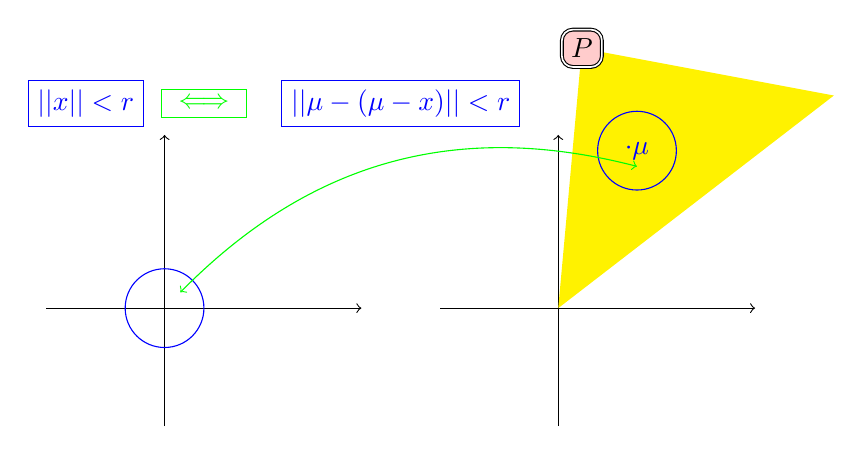
\begin{tikzpicture}
	
          

		%Dibuja los ejes figura 1
		\draw[->] (-1.5,0) -- (2.5,0);
		\draw [->] (0,-1.5) -- (0,2.2);
		%Circulo de figura 1 
		 \draw[color=blue] (0,0) circle (0.5cm);
		
			%Dibuja los ejes figura 2
		\draw[->] (3.5,0) -- (7.5,0);
		\draw [->] (5,-1.5) -- (5,2.2);
		
			%%%Crea el cono P en la figura 2 %%%
		\fill[fill=yellow]
		(5,0)
		-- (8.5,2.7) 
		-- (5.3,3.3) node[fill=red!20,draw,double,rounded corners] {$ P $};
		%Circulo en la figura 2
		\draw[color=blue] (6,2) circle (0.5cm);
		 \node[ color=blue] (2) at (6,2) { $ \cdot  \mu  $};
		%Linea verde que une figurta 1 y figura 2 
      \draw[<->,color=green] (0.2,0.2) to[bend left] (6,1.8);
      
      
      
      \node[draw, color=blue] (2) at (-1,2.6) { $|| x || < r $};
      \node[draw, color=green] (3) at (0.5,2.6) { $ \iff  $};
      \node[draw, color=blue] (4) at (3,2.6) { $ || \mu - (\mu - x) || < r $};
   
\end{tikzpicture}
	
	
	
	\end{itemize}
\end{frame}






%%%%%%%%%%%%%%%%%%%%%%%%%%%%%%%%%%%%%%%%%%%%%%%%%%%%%%%%%%%%%%%%%%%%%%%%%%%%%%%%%%%%%%%%%%%%%%%%%%%%%%%%%%%%%%%%%%%%%%%%%%%%%%%%%%%%%%%%%%%%%%%%%%%%%%%%%%%%%%%%%%%%%%%%%%%%%%%%%%%%%%%%%%%%%%%%%%%%%%%%%%%%%%%%%%%%%%%%%%%%%%%%%%%%%%%%%%%%%%%%%%%%%%%%%%%%%%%%%%%%%%%%%%%%%%%%%%%%%%%%%%%%%%%%%%%%%%%%%%%%%%%%%%%%%

\begin{frame}{}
    \begin{itemize}
        \item \textbf{Ejemplo:} Un espacio sin esfera acotada que cumple la descomposición de Jordan. 
        \begin{block}{}
            	$ (l^{1}, || \cdot ||_{1} ) $ con $l^{1}_{+} = \{ \{a_{n} \} \in l^{1} : a_{n} \geq 0 \mbox{ para todo } n \in \mathbb{N} \} $ cumple la descomposición de Jordan.
        \end{block}
        	Sea $f:[a,b]\rightarrow l^{1}$ uy $f_{j} :[a,b]\rightarrow \mathbb{R} $ con $ j \in \mathbb{N} $ tal que para  $t\in [a,b]$
		\[f(t)=\sum_{j=1}^{\infty} f_{j}(t)e_{j} , \]
		donde $ e_{j} $ es un vector unitario sobre
	 $l^{1}$.\\	
	 Si  $f$ es v. a., entonces $ f_{j} $ es v. a. y $ f_{j} (x) = V (f_{j}, [a,x] ) - [ V (f_{j}, [a,x] ) - f_{j} (x) ] $. 
	
	
    \end{itemize}
\end{frame}

\begin{frame}{}
    $ \{ V (f_{j}, [a,x] ) \} \in l^{1} $ ya que  $ 0 \leq  V (f_{j}, [a,x] ) \leq  V (f_{j}, [a,b] ) $ y así $ \sum_{j=1}^{\infty} V (f_{j}, [a,x] ) \leq \sum_{j=1}^{\infty}  V (f_{j}, [a,b] ) \leq V (f, [a,b] ) $.
	
	Por tanto,  $$ f_{2}(x) = \{ V (f_{j}, [a,x] ) \} , \  f_{1} (x) = \{ V (f_{j}, [a,x] ) - f_{j} (x) \} \in l^{1} $$
 y así
 $f= f_{2} - f_{1}$.
\end{frame}
